\namedsection{Frameworks}{J}
Für jedes Problem gibt es das passende Handwerkszeug. Es ist nicht nachhaltig jedes benötigte Versatzstück erneut zu implementieren, wenn es bereits ein passendes dazu gibt. In den folgenden Abschnitten wollen wir demzufolge herausfinden welches Framework unsere Anforderungen an die Architektur, Produktivität und vorhandenen Erfahrungen am Besten abdeckt.

\namedsubsection{Evaluierungskriterien}{J}
Für jedes Kriterium werden wir kurz beschreiben was es bedeutet und anschließend ausführen warum es für unser Projekt von Bedeutung ist.
\begin{description}
    \item [Performanz]
    Wie performant ist die Technologie?
    Wie verhält sich die Technologie bei der Verarbeitung von großen Datensätzen?
    Wie gut ist das Handling für High Throughput von I/O-Aufgaben?
    Wenn der Durchsatz hoch ist, können mehr I/O-Aufgaben pro Zeiteinheit bewältigt werden was der Skalierbarkeit zugute kommt.
    \item [Komplexität]
    Wie komplex ist die dafür benötigte Infrastruktur und Setup?
    Wie groß ist  der Einarbeitungsaufwand in die Technologie?
    Eine Einarbeitung in eine riesige Microservice-Landschaft mit dutzenden Services erfordert mehr Zeit als ein Monolith. Ähnlich verhält es sich mit den Infrastrukturaufwand.
    \item [Dokumentation / Community]
    Wie qualitativ ist die offizielle Dokumentation?
    Wie groß und aktiv ist die Community?
    Wie viel zusätzliches Lernmaterial ist öffentlich verfügbar?
    Bei genügend Beispielen und eine aktive Community verkürzt es die Einarbeitungszeit.
    \item [Team Know-How]
    Wie viel Vorwissen haben die Teammitglieder mit der Technologie?
    Bereits vorhandenes Wissen nutzen um effizienter zu einer Lösung kommen zu können.
    \item [Skalierbarkeit]
    Wie gut lässt sich die Applikation skalieren?
    Wie sehr ist die Technologie für Enterprise-Projekte geeignet?
    Kommt das Framework bereits mit vordefinierten Lösungen für Microservice-Architekturen, dann erleichtert es den Aufbau einer eigenen modularen Softwarearchitektur.
\end{description}

\namedsubsection{Betrachtete Frameworks}{J}
In diesem Bereich untersuchen wir der Reihe nach die Frameworks Spring (Boot), Loopback, Express, Flask, Slim
und .NET. Der Aufbau enthält jeweils eine Beschreibung und spezifische Charakteristika des Frameworks und endet schließlich in einer Zusammenfassung der Vorteile und Nachteile.

\subsubsection*{Spring\hfill[J]}
Spring ist ein modulares, quelloffenes Java-Framework mit dem Ziel, die Entwicklung von Java/Java EE zu vereinfachen und gute Programmierpraktiken zu fördern.

\begin{figure}[!h]
\centering
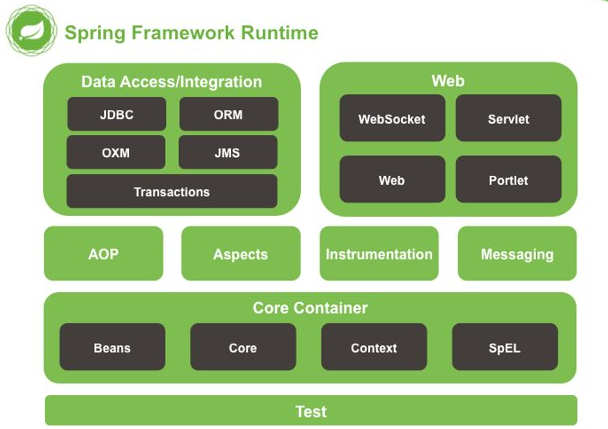
\includegraphics[width=9cm]{images/0x_technology_stack/spring_framework_runtime.png}
\caption{Spring Framework Runtime \cite{springruntime}}
\end{figure}

Spring Boot ist ein Framework zur Entwicklung von allein lauffähigen, für den produktiven Einsatz geeigneten Spring-basierten Applikationen ("convention over configuration") und benötigt keinen Applikationsserver, sondern wird als Fat-Jar-Artefakt inklusive einem eingebetteten Webserver (z.B. Apache Tomcat/Netty) ausgeliefert. Somit wird bereits ein großteil der sonst notwendigen Arbeitsschritte vom Framework selbst übernommen.

Es basiert auf Java ist modular und flexibel aufgebaut. Als Open Source Framework das bereits sehr lange existiert hat es auch eine große Community. Allein das Hauptrepository vereint bereits 20.000 Commits und 414 Contributors auf sich.

\subsubsection*{Vorteile}
\begin{itemize}
    \item Sehr gute Dokumentation und sehr große Community
    \item Umfangreiches Ökosystem mit vielen Libraries
    \item Eignung für CPU-intensive Aufgaben durch Multithreading
    \item Bietet API für Non-blocking I/O für High Throughput Applikationen bei geringer Ressourcennutzung an
    \item JVM ist sicher und hat sich über die Jahre bereits bewährt
    \item Bessere Performance als Skriptsprachen, da der JVM mehrere Metadaten während der Runtime zur Verfügung stehen
    \item Enterprise Support über Pivotal verfügbar
    \item Enterprise Ready Framework
\end{itemize}

\subsubsection*{Nachteile}
\begin{itemize}
    \item Java code ist verbose und es ist viel Boilerplate Code im Vergleich zu anderen Technologien erforderlich
    \item Komplexes Framework, welches Einarbeitung erforderlich macht
\end{itemize}

\subsubsection*{Loopback 4\hfill[J]}
Ein von IBM entwickeltes Enterprise Framework, dass auch in der Cloud gut lauffähig ist. Das Framework ist kompatibel zu Express Middlewares und profitiert so von einem bereits umfangreichen Ökosystem. Versucht zudem durch "Convention over Configuration" den Aufwand bei Entwicklungsarbeiten zu reduzieren.

Grundsätzlich wird TypeScript für das Framework benutzt aber es ist auch möglich darauf zu verzichten und JavaScript zu nutzen. Allerdings wird es nicht empfohlen. Insgesamt ist Loopback 4 wie Spring auch, sehr modular und flexibel aufgebaut. Genauso ist Loopback 4 auch als Open Source Projekt konzipiert ist jedoch bedeutend jünger. Das Hauptrepository umfasst gerade mal 2.900 Commits und 104 Contributors.

\begin{figure}[!h]
\centering
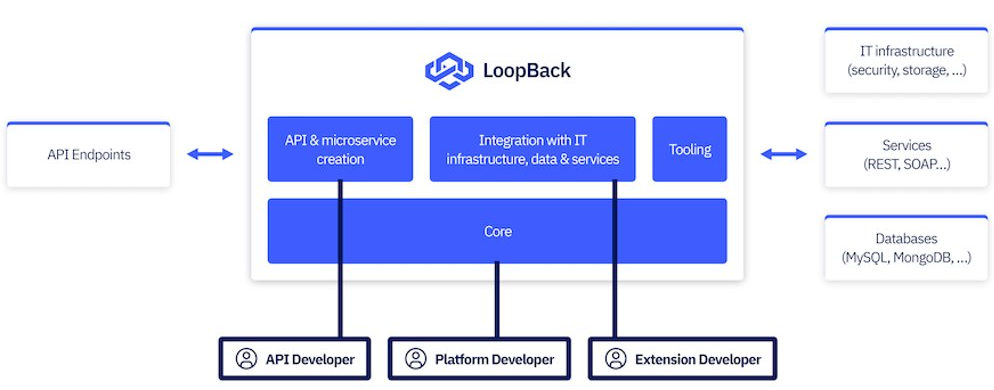
\includegraphics[width=13cm]{images/0x_technology_stack/loopback_4.png}
\caption{Loopback 4 Diagramm \cite{loopback4}}
\end{figure}

\subsubsection*{Vorteile}
\begin{itemize}
    \item Gute Erweiterbarkeit durch Express.js Middlewares
    \item Konnektoren für Datenbankanbindung sind bereits vorhanden
    \item Hohe Modularisierung durch SOA
    \item Weniger Fehleranfällig als reine JavaScript Applikationen, da TypeScript Fehler bereits beim kompilieren abfängt
    \item Schnelle Ergebnisse mit überschaubaren Programmieraufwand
    \item Zugriff auf das größte Package Repository aller Sprache; derzeit über 1 Millionen Packages verfügbar
\end{itemize}

\subsubsection*{Nachteile}
\begin{itemize}
    \item Junges Framework (2018)
    \item Einarbeitung in Framework spezifische Logik notwendig
    \item Performance-Nachteile, da basierend auf High Level Programmiersprache
    \item Relativ kleine Community (2398 commits)
\end{itemize}

\subsubsection*{Express\hfill[Filip]}
Express ist ein minimalistisches open source Webframework für Javascript mit starkem Fokus auf Flexibilität im Ansatz von benutzerdefinierten, im Gegensatz zu standardisierten, bewährten Vorgehensweisen. Es ist Teil des aktuell größten Ökosystem aller Programmiersprachen - Node.js und ist mit über 47.000 Sterne, 5.500 Commits und 230 Contributors in dem Hauptrepository das größte aller in Node.js verfügbaren Webframeworks.

Es basiert auf einer modularen Architektur mit individuellen Funktionalitäten, die als Plugins verfügbar sind. Zu den wichtigsten Merkmalen gehören eine große Auswahl an Template Engines, robustes Routing und hohe I/O-Performanz.

\subsubsection*{Vorteile}
\begin{itemize}
    \item Große Community und gute Dokumentation
    \item Zugriff auf das größte Package Repository aller Sprache; derzeit über 1
Millionen Packages verfügbar
    \item Für das Erstellen von APIs ausgelegt
    \item Gut geeignet für das Handling von High Throughput I/O
    \item Stark reduziertes Boilerplate Code
    \item Einfache Integration von NoSQL-Datenbanken
    \item JSON ist Subset von JavaScript
    \item Kein Kompilierungsschritt notwendig, was zu schnelleren Entwicklungszeiten führt
\end{itemize}

\subsubsection*{Nachteile}
\begin{itemize}
    \item Performance-Verlust, da High-Level Programmiersprache
    \item Für CPU intensive Aufgaben schlecht geeignet
    \item Mehr Runtime Errors sind möglich
\end{itemize}

\subsubsection*{Flask\hfill[Filip]}
Flask ist ein minimalistisches, Python basiertes open source Webframework. Einfachheit, stark reduziertes Boilerplate code und schnelle Entwicklung von Prototypen sind seine wichtigste Merkmale. Sehr hohe Flexibilität und Erweiterbarkeit ist durch Teilung in sehr granulare individuelle Komponente erreicht. Dieser Ansatz resultiert aber in erhöhtem Aufwand – mehr Entscheidungen sind selbst dem Entwickler gelassen.

Das Framework profitiert von einem großem und aktivem Community – das Projekt Repository umfasst gerade mal über 3.800 Commits und über 560 Contributors.

\subsubsection*{Vorteile}
\begin{itemize}
    \item Gute Dokumentation
    \item Für rapid Prototyping geeignet
    \item Schnelle Lernkurve
    \item Leicht erweiterbar
\end{itemize}

\subsubsection*{Nachteile}
\begin{itemize}
    \item Relativ kleine Community
    \item Weniger 'Out of the Box' Funktionalität
    \item Keine gute ORM Mapping Unterstützung
    \item Erbt Python-bezogene Performanzprobleme
\end{itemize}

\subsubsection*{Slim\hfill[Filip]}
Slim ist ein PHP basiertes open source Micro-WebFramework. Es unterstützt alle gemeinsame Szenarien, eignet sich aber besonders gut für APIs Entwicklung und für Rapid Prototyping. Ähnlich zu Python Flask sind bei Slim Einfachheit und Geschwindigkeit der Entwicklung große Vorteile. Die Reichheit an Bibliotheken ist jedoch nicht so groß relativ zu anderen bewerteten Frameworks – für die Projektumsetzung besonders relevant sind die ORM tools die im Slim noch nicht ausgereift sind.

Das Framework verfügt über eine relativ aktive, wenn nicht so große Community. Das Repository fasst aktuell etwa 4.000 Commits von fast 200 Contributors um.
\subsubsection*{Vorteile}
\begin{itemize}
    \item Gute Dokumentation
    \item Für rapid Prototyping geeignet
    \item Einbinden von Drittanbietern über Packagist möglich
    \item Leichte und schnelle Einarbeitung
\end{itemize}

\subsubsection*{Nachteile}
\begin{itemize}
    \item Relativ kleine Community
    \item Keine gute ORM Mapping Unterstützung
    \item ORM Mapping tools nicht komplett ausgereift
\end{itemize}

\subsubsection*{ASP.NET\hfill[Filip]}
ASP.NET ist ein etabliertes, open source, C\# basiertes Framework, das von Microsoft entwickelt wurde und auf der MVC Architektur basiert. Seine wichtigste Designziele sind Skalierbarkeit, Performanz und Sicherheit.

Das Framework profitiert von einer sehr großen und aktiven Community. Das Hauptrepository verfügt aktuell über ca.  Sterne, 40.700 Commits und 670 Contributors.

\begin{figure}[!h]
\centering
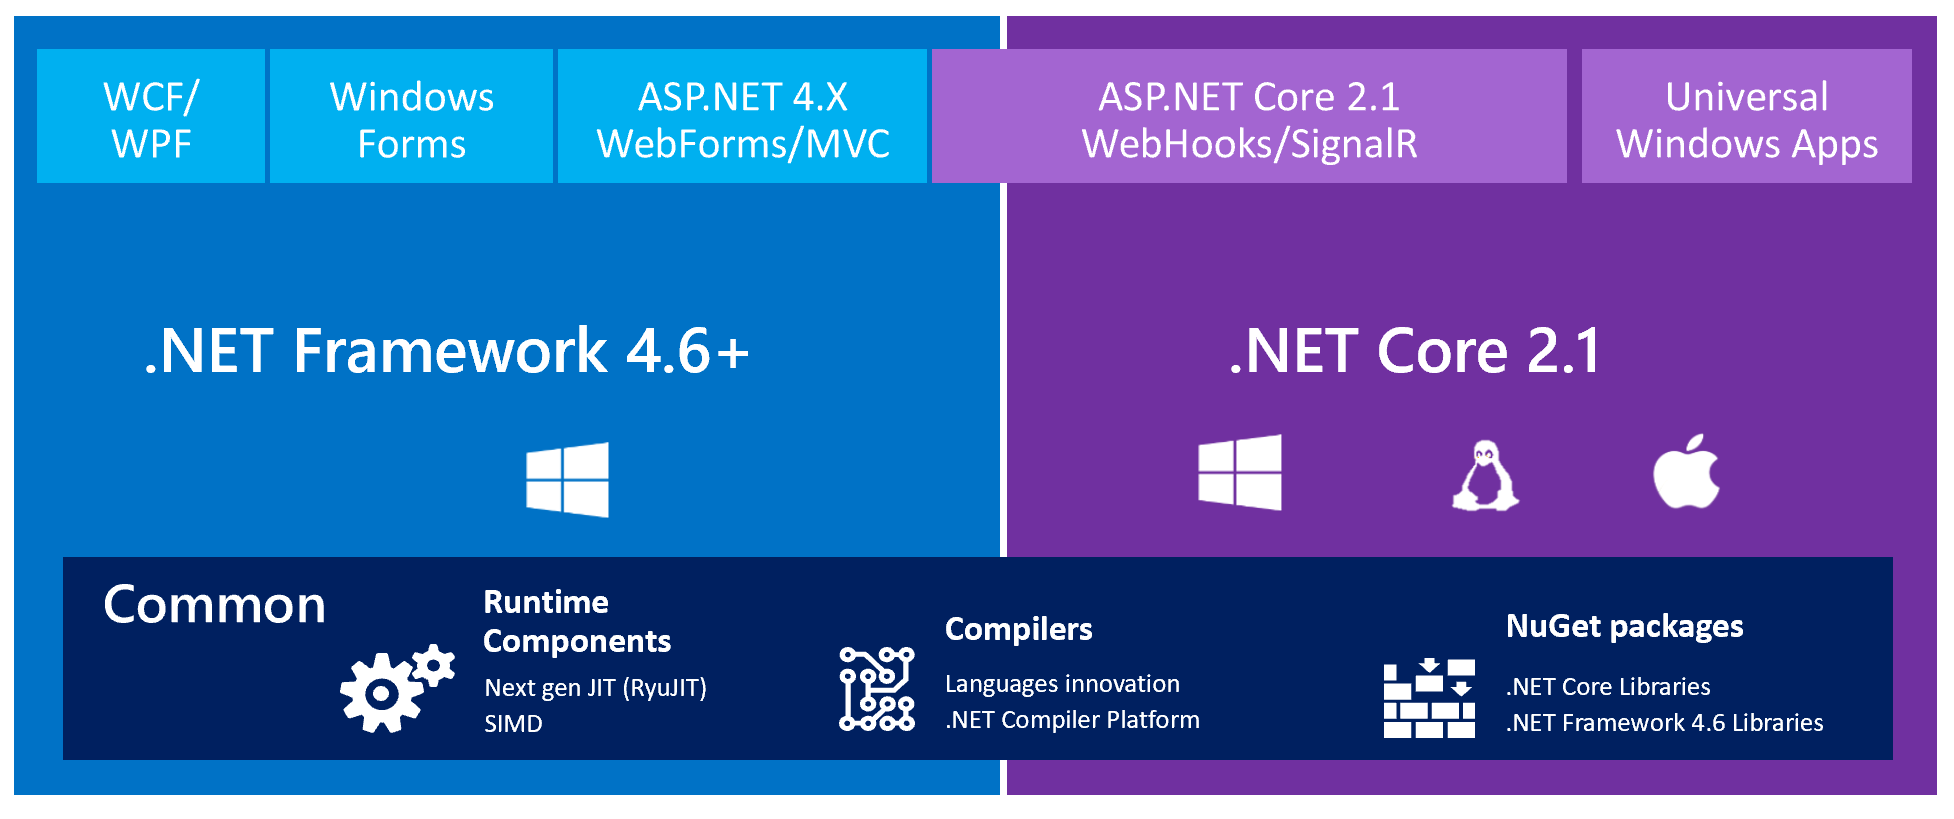
\includegraphics[width=11cm]{images/0x_technology_stack/asp_net.png}
\caption{ASP.NET}
\end{figure}
\subsubsection*{Vorteile}
\begin{itemize}
    \item Sehr große Community und gute Dokumentation
    \item Reiche Funktionalität ohne zusätzlichen Libraries
    \item Einfachere Fehlererkennung und hohe Robustheit wegen starker Typisierung
    \item Enterprise Support vorhanden
\end{itemize}

\subsubsection*{Nachteile}
\begin{itemize}
    \item ORM Mapping nicht flexibel genug
    \item Viele Libraries sind komerziell
\end{itemize}

\namedsubsection{Auswertung und Diskussion}{J}
Aus der Tabelle \ref{fig:framework_evaluation} kann unsere Auswertung entnommen werden. Die Zuteilung der Sterne hat sich aus der Gewichtung der Vor- und Nachteile der jeweiligen Frameworks ergeben. In den folgenden Absätzen werden wir einen Überblick auf hoher Ebene geben. Ziel war es die wichtigsten Gründe für oder gegen einzelne untersuchte Frameworks benannt zu haben.

Spring Boot bewährt sich seit Jahrzehnten im Enterprise-Umfeld. Es bietet reichlich getestete Komponenten zur Erweiterung inklusive Security. Darüber hinaus existiert hier die meiste Erfahrung im Team und eine umfangreiche Dokumentation mit zahlreichen Beispielen und Bootstrap-Projekten. Zudem ist Java bei der Performance für CPU-intensiven Aufgaben, zusammen mit C\#, am stärksten. Direkte Datenbankverbindungen ist ebenfalls ein starker Bereich in Java. JDBC schlägt teilweise sogar ODBC, das in C geschrieben ist.

\begin{table}[]
\centering
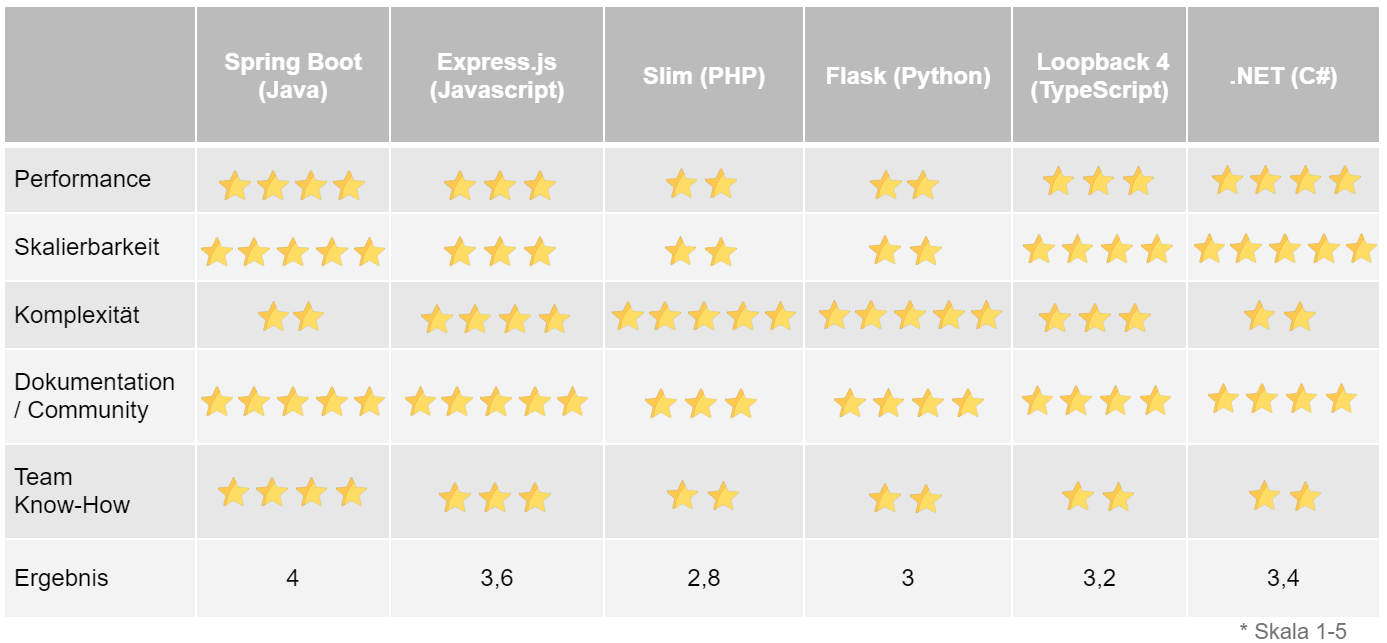
\includegraphics[width=16cm]{images/0x_technology_stack/frameworks_comparision_table.png}
\caption{Framework Auswertung}
\label{fig:framework_evaluation}
\end{table}

Express.js, Slim und Flask sind mehr wie Microframeworks die vor allem das Grundgerüst für das Entwickeln von APIs bereitstellen. Dazu gehört unter anderem das Routing und Middlewares. Demnach müssen einige Bestandteile entweder über Packages bezogen, falls überhaupt vorhanden, oder selbst programmiert werden.

Loopback 4 bietet zwar viele Bausteine an, die für eine Datenintegration relevant sind, allerdings ist das Projekt noch ziemlich jung (2018). Ferner hat es speziell im CPU-lastigen Bereich das Nachsehen im Vergleich zu Java wie aus dem Abschnitt zu den Programmiersprachen zu entnehmen ist.

Alles rund um das .NET Ökosystem ist insbesondere aufgrund der kaum vorhandenen Erfahrungen im Team nicht relevant für uns.
